\section{Konstrukion mit Zirkel und Lineal}

\textbf{Aufgabe}: Sei $M \subset \mathbb{C} = \mathbb{R}^2$, z.B.:
$M=\{0,1\}$.
\[\mbox{Linien: }\mathcal{L}(M) \defeqr \{L \subset \mathbb{R}^2 \mbox{ Gerade: }
|L \cap M| \geq 2\}\; \cup \;\{K_{z_1 - z_2}(z_3): z_1, z_2, z_3
\in M\}\qquad\qquad\] $(K_r(z) = \{y \in \mathbb{R}^2:\;|z-y| =
r\}) \\\\ K_1(M) \defeqr \{z \in \mathbb{C}:\; z$ liegt auf zwei
verschiedenen Linien in $\mathcal{L}(M)\}\\$ $K_n(M) \defeqr
K_1(K_{n-1}(M))$ für $n \geq 2\\$ $K(M) \defeqr \bigcup_{n=1}^\infty
K_n(M)$
\newline\newline\textbf{Beobachte}: $M \subseteq K_1(M)$,
falls $|M| \geq 2$.
\newline \textbf{Ab jetzt}: $0,1 \in M$, $M$ symmetrisch zur $x-$Achse (dh.
für $z = x+iy \in M$ ist auch $\bar z = x -iy \in M$

\begin{Bem}
Für jedes $z \in K_1(M)$ ist
$[\mathbb{Q}(M)(z) : \mathbb{Q}(M)] \leq 2$

\bew{\newline Vorüberlegung: Für $z \in M$ ist $\Re(z) =
\frac{1}{2}(z+\bar z) \in \mathbb{Q}(M)$ und $\Im(z) = \frac{1}{2}(z
-\bar z) \in \mathbb{Q}(M).$} {
\item $z$ ist Schnittpunkt zweier Geraden in $\mathcal{L}(M) \Ra
z$ ist Lösung zweier linearer Gleichungen $z_1 + \lambda z_2 = z_1'
+ \mu z_2'$
\item $z$ ist Schnittpunkt einer Geraden und eines Kreises: $\Ra$
quadratische Gleichung mir Koeffizienten in $\mathbb{Q}(M)$
\item $z$ ist Schnittpunkt zweier Kreise $K_{r_1}(m_1)$ und
$K_{r_2}(m_2)$ mit Mittelpunkten $m_1,m_2 \in M$. Radien: $r_1 =
|z_1 - z_1'|$, $r_2 = \dots$ also $r_1^2 = (z_1 - z_1') (\overline{z_1 -
z_1'}) \in \mathbb{Q}(M)$.

Dann ist $|z-m_1|^2 = r_1^2$.

$\Ra z\bar z - (z\bar{m_1} + \bar z m_1) = r_1^2 - m_1 \bar{m_1}$
und $z \bar z - (z \bar{m_2} + \bar z m_2) = r_2^2 - m_2 \bar{m_2}
\Ra 2 \Re[z(\bar{m_1} - \bar{m_2})] = r_1^2 - r_2^2 - (m_1 \bar{m_1}
- m_2 \bar{m_2})$

Das ist eine lineare Gleichung, die $\Re(z)$ und $\Im(z)$ enthält.
Einsetzen in $(1)$ ergibt quadratische Gleichung für $\Re(z)$ (mit
Koeffizienten in $\mathbb{Q}(M)$)}
\end{Bem}

\begin{Satz}
\begin{enum}
\item $K(M)$ ist algebraische Körpererweiterung von $\mathbb{Q}(M)$
\item Sei $L/\mathbb{Q}(M)$ endliche Körpererweiterung. Gibt es $n
\geq 0$ und Körper $\mathbb{Q}(M) = L_0 \subset L_1 \subset \dots
\subset L_n = L$, mit $[L_i : L_{i-1}] = 2$ für $i=1,\dots,n$, dann
ist $L \subseteq K(M)$.
\end{enum}

\sbew{1.0}{
Seien $a,b \in K(M)$. Zu zeigen: $a+b, -a, a \cd b, \frac{1}{a} \in
K(M)$.\newline
$a+b \in K(M):$
\begin{center}
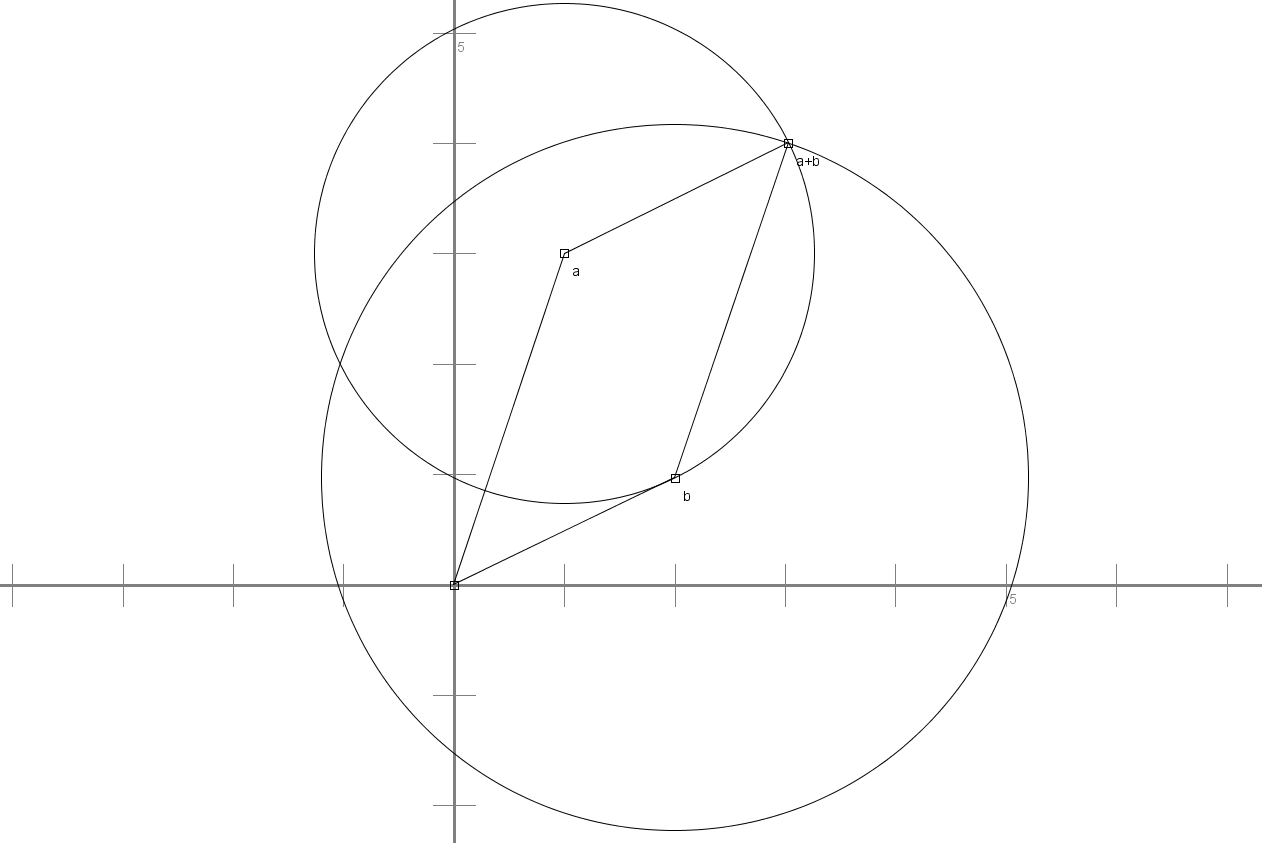
\includegraphics[width=\textwidth]{alg16a1.png}
\end{center}
}

\sbew{1.0}{
$-a \in K(M):$
\begin{center}
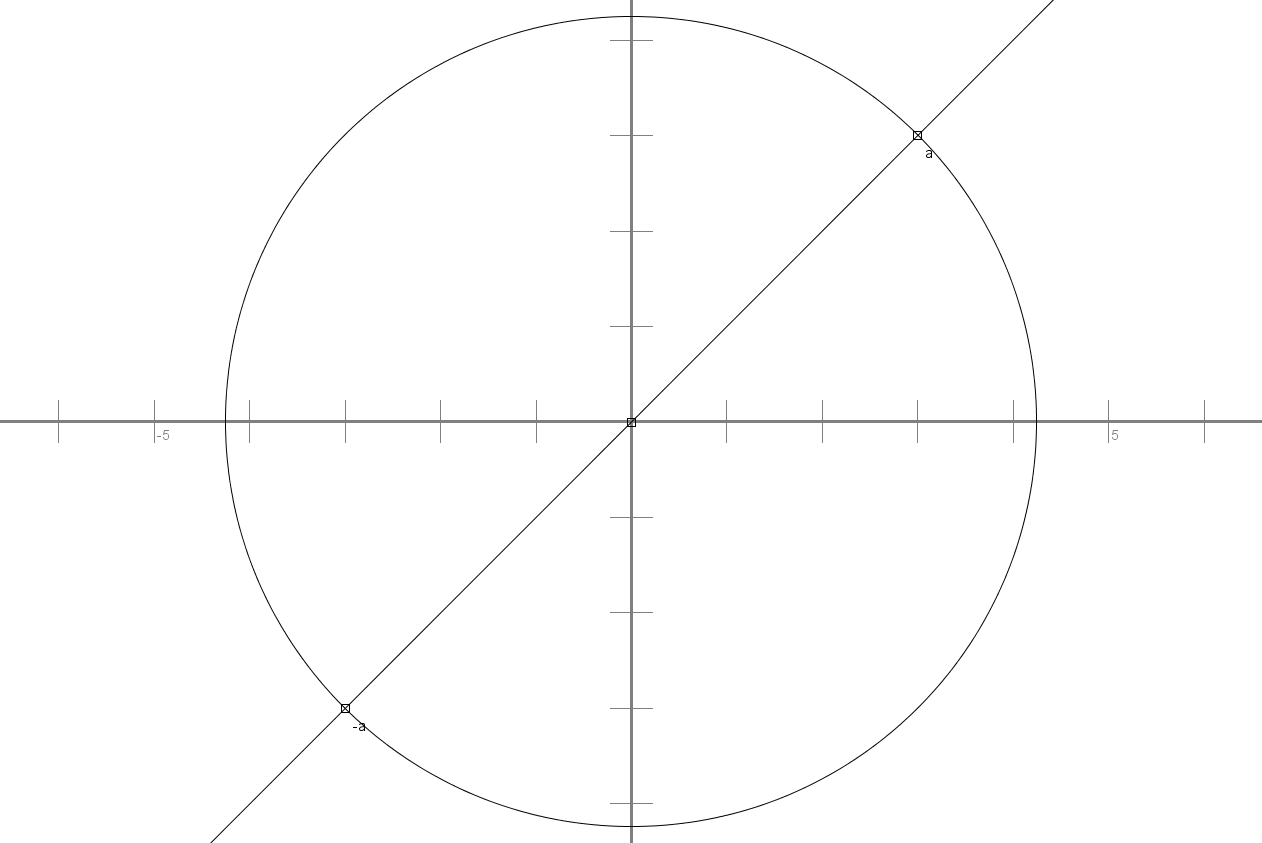
\includegraphics[width=\textwidth]{alg16a2.png}
\end{center}
}

\sbew{1.0}{
$a \cd b \in K(M):$\newline
Strahlensatz: $\frac{1}{a} = \frac{b}{x}$, also $x = a \cd b$. Winkel addieren
$\chk \Ra a \cd b$ allgemein $\chk$
\begin{center}
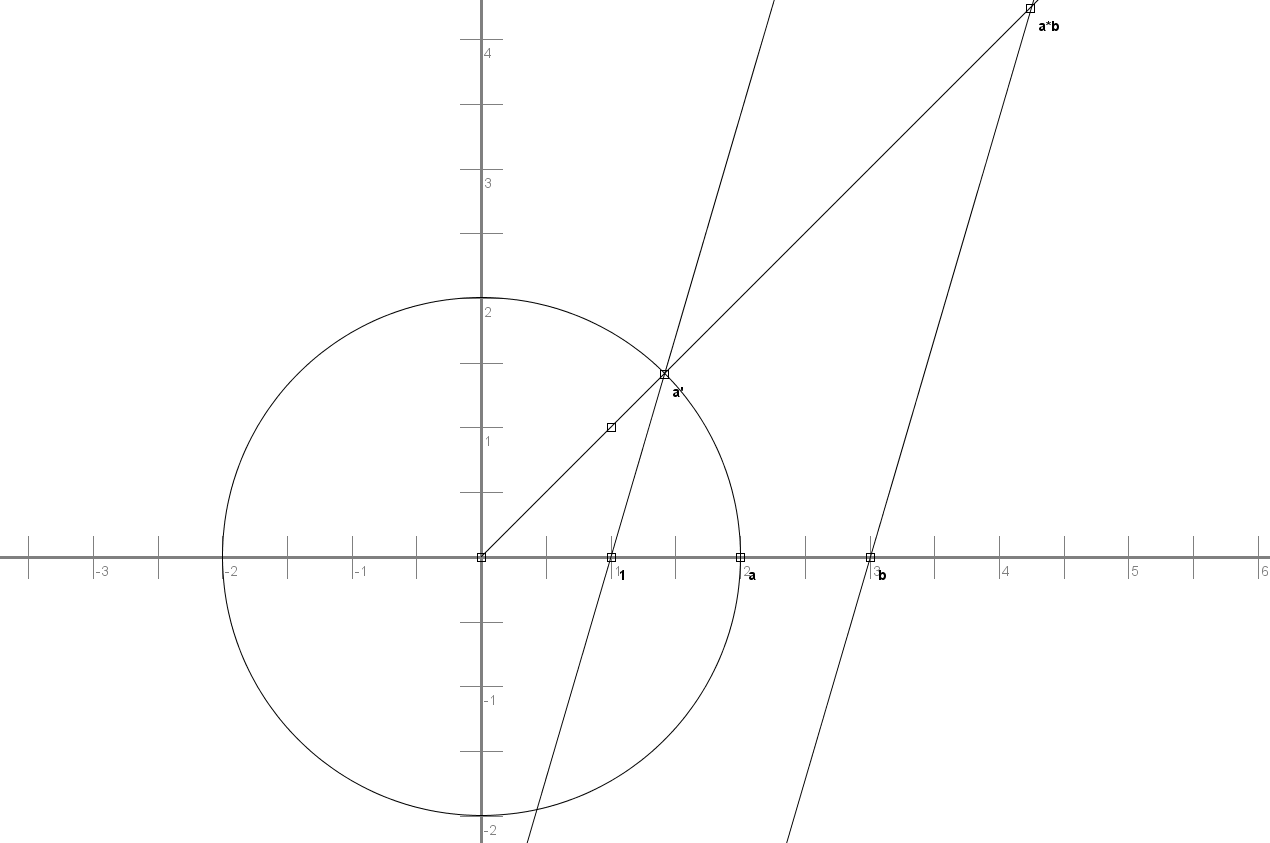
\includegraphics[width=\textwidth]{alg16a3.png}
\end{center}
}

\sbew{1.0}{
$\frac{1}{a} \in K(M):$ \OE $a \in \mathbb{R}$
\begin{center}
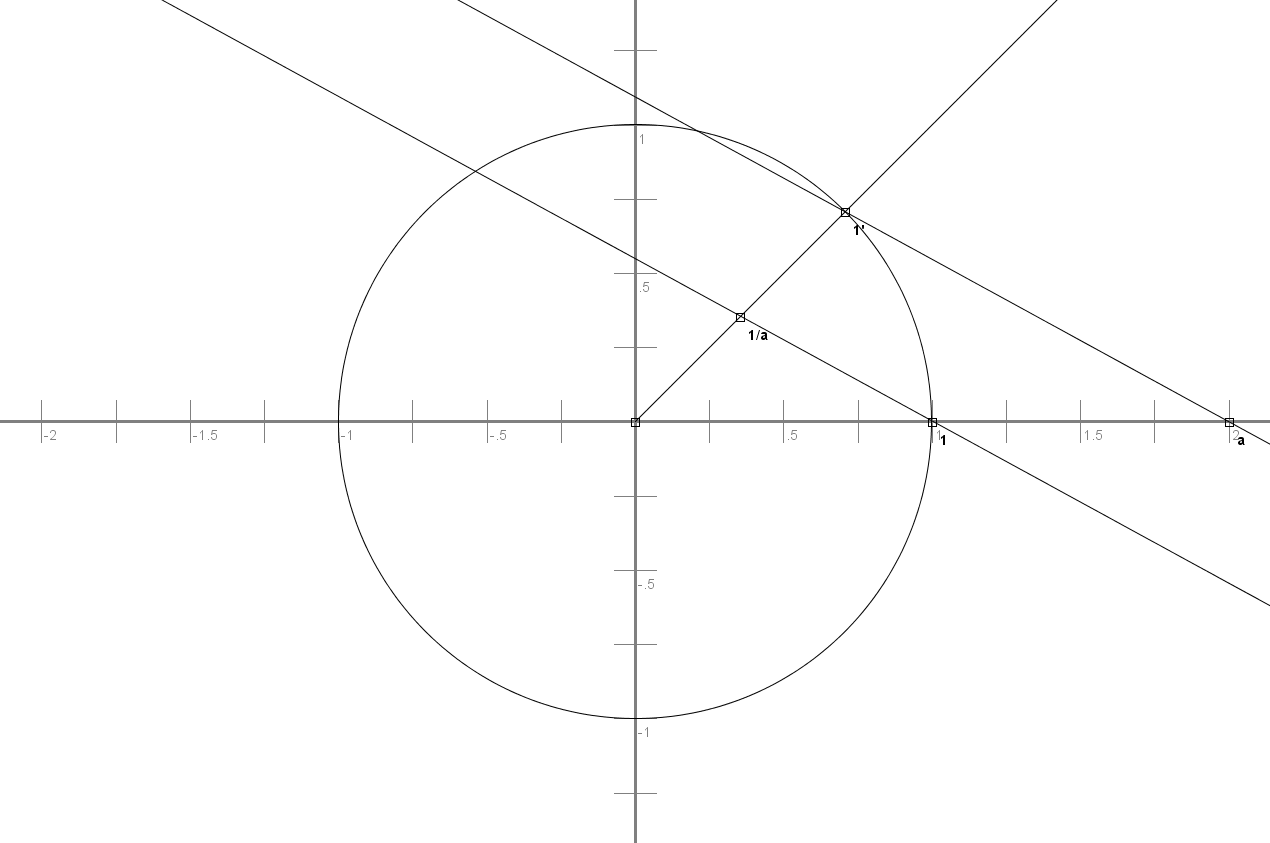
\includegraphics[width=\textwidth]{alg16a4.png}
\end{center}
}

\sbew{1.0}{
Wurzelziehen: $a \in \mathbb{R}$
\begin{center}
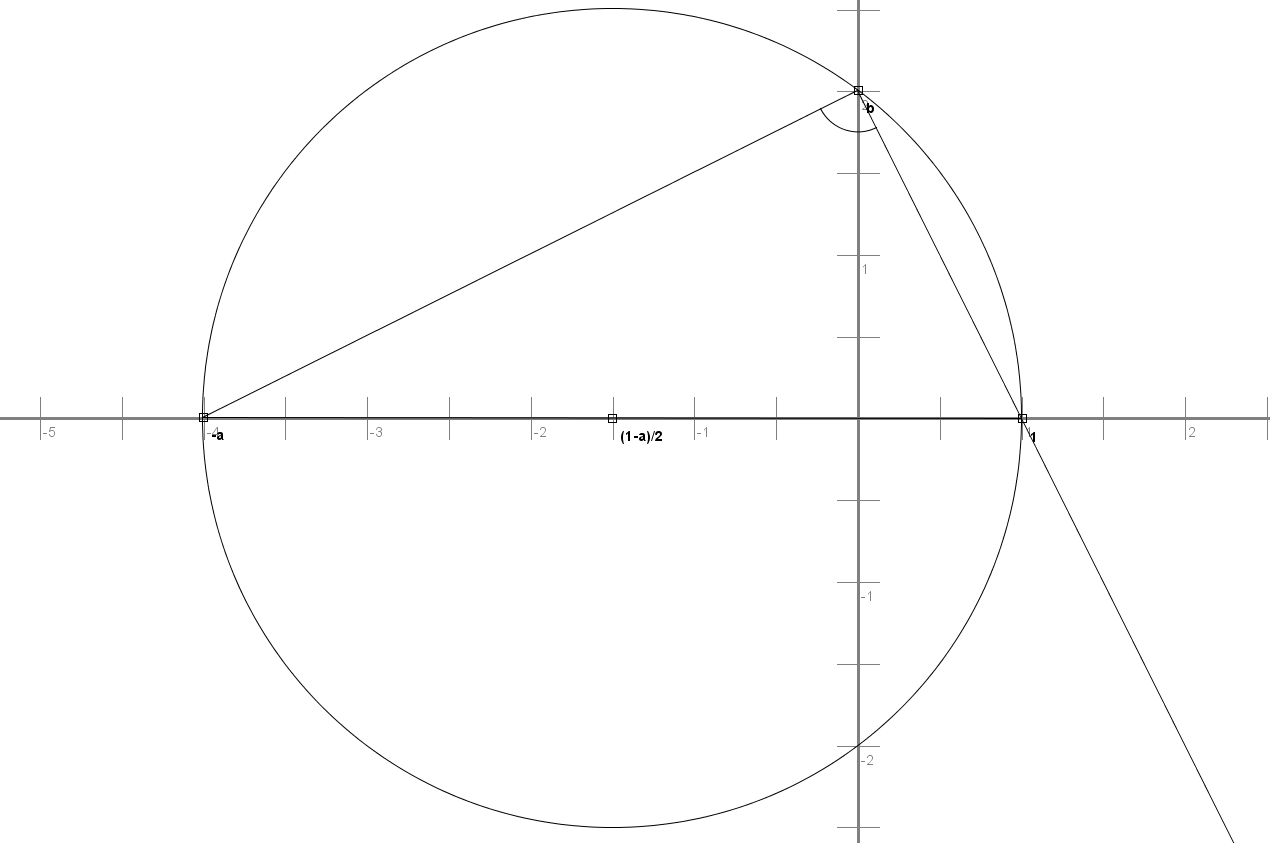
\includegraphics[width=\textwidth]{alg16b.png}
\end{center}
$\overset{\scriptsize\mbox{Thales}}{\Ra}$ Winkel ist rechtwinklig
$\overset{\scriptsize\mbox{Höhensatz}}{\Ra} b^2=|-a| \cd 1 = a$
}
\end{Satz}
